% Options for packages loaded elsewhere
\PassOptionsToPackage{unicode}{hyperref}
\PassOptionsToPackage{hyphens}{url}
%
\documentclass[
  man]{apa7}
\usepackage{amsmath,amssymb}
\usepackage{iftex}
\ifPDFTeX
  \usepackage[T1]{fontenc}
  \usepackage[utf8]{inputenc}
  \usepackage{textcomp} % provide euro and other symbols
\else % if luatex or xetex
  \usepackage{unicode-math} % this also loads fontspec
  \defaultfontfeatures{Scale=MatchLowercase}
  \defaultfontfeatures[\rmfamily]{Ligatures=TeX,Scale=1}
\fi
\usepackage{lmodern}
\ifPDFTeX\else
  % xetex/luatex font selection
\fi
% Use upquote if available, for straight quotes in verbatim environments
\IfFileExists{upquote.sty}{\usepackage{upquote}}{}
\IfFileExists{microtype.sty}{% use microtype if available
  \usepackage[]{microtype}
  \UseMicrotypeSet[protrusion]{basicmath} % disable protrusion for tt fonts
}{}
\makeatletter
\@ifundefined{KOMAClassName}{% if non-KOMA class
  \IfFileExists{parskip.sty}{%
    \usepackage{parskip}
  }{% else
    \setlength{\parindent}{0pt}
    \setlength{\parskip}{6pt plus 2pt minus 1pt}}
}{% if KOMA class
  \KOMAoptions{parskip=half}}
\makeatother
\usepackage{xcolor}
\usepackage{graphicx}
\makeatletter
\def\maxwidth{\ifdim\Gin@nat@width>\linewidth\linewidth\else\Gin@nat@width\fi}
\def\maxheight{\ifdim\Gin@nat@height>\textheight\textheight\else\Gin@nat@height\fi}
\makeatother
% Scale images if necessary, so that they will not overflow the page
% margins by default, and it is still possible to overwrite the defaults
% using explicit options in \includegraphics[width, height, ...]{}
\setkeys{Gin}{width=\maxwidth,height=\maxheight,keepaspectratio}
% Set default figure placement to htbp
\makeatletter
\def\fps@figure{htbp}
\makeatother
\setlength{\emergencystretch}{3em} % prevent overfull lines
\providecommand{\tightlist}{%
  \setlength{\itemsep}{0pt}\setlength{\parskip}{0pt}}
\setcounter{secnumdepth}{-\maxdimen} % remove section numbering
% Make \paragraph and \subparagraph free-standing
\ifx\paragraph\undefined\else
  \let\oldparagraph\paragraph
  \renewcommand{\paragraph}[1]{\oldparagraph{#1}\mbox{}}
\fi
\ifx\subparagraph\undefined\else
  \let\oldsubparagraph\subparagraph
  \renewcommand{\subparagraph}[1]{\oldsubparagraph{#1}\mbox{}}
\fi
\newlength{\cslhangindent}
\setlength{\cslhangindent}{1.5em}
\newlength{\csllabelwidth}
\setlength{\csllabelwidth}{3em}
\newlength{\cslentryspacingunit} % times entry-spacing
\setlength{\cslentryspacingunit}{\parskip}
\newenvironment{CSLReferences}[2] % #1 hanging-ident, #2 entry spacing
 {% don't indent paragraphs
  \setlength{\parindent}{0pt}
  % turn on hanging indent if param 1 is 1
  \ifodd #1
  \let\oldpar\par
  \def\par{\hangindent=\cslhangindent\oldpar}
  \fi
  % set entry spacing
  \setlength{\parskip}{#2\cslentryspacingunit}
 }%
 {}
\usepackage{calc}
\newcommand{\CSLBlock}[1]{#1\hfill\break}
\newcommand{\CSLLeftMargin}[1]{\parbox[t]{\csllabelwidth}{#1}}
\newcommand{\CSLRightInline}[1]{\parbox[t]{\linewidth - \csllabelwidth}{#1}\break}
\newcommand{\CSLIndent}[1]{\hspace{\cslhangindent}#1}
\ifLuaTeX
\usepackage[bidi=basic]{babel}
\else
\usepackage[bidi=default]{babel}
\fi
\babelprovide[main,import]{english}
% get rid of language-specific shorthands (see #6817):
\let\LanguageShortHands\languageshorthands
\def\languageshorthands#1{}
% Manuscript styling
\usepackage{upgreek}
\captionsetup{font=singlespacing,justification=justified}

% Table formatting
\usepackage{longtable}
\usepackage{lscape}
% \usepackage[counterclockwise]{rotating}   % Landscape page setup for large tables
\usepackage{multirow}		% Table styling
\usepackage{tabularx}		% Control Column width
\usepackage[flushleft]{threeparttable}	% Allows for three part tables with a specified notes section
\usepackage{threeparttablex}            % Lets threeparttable work with longtable

% Create new environments so endfloat can handle them
% \newenvironment{ltable}
%   {\begin{landscape}\centering\begin{threeparttable}}
%   {\end{threeparttable}\end{landscape}}
\newenvironment{lltable}{\begin{landscape}\centering\begin{ThreePartTable}}{\end{ThreePartTable}\end{landscape}}

% Enables adjusting longtable caption width to table width
% Solution found at http://golatex.de/longtable-mit-caption-so-breit-wie-die-tabelle-t15767.html
\makeatletter
\newcommand\LastLTentrywidth{1em}
\newlength\longtablewidth
\setlength{\longtablewidth}{1in}
\newcommand{\getlongtablewidth}{\begingroup \ifcsname LT@\roman{LT@tables}\endcsname \global\longtablewidth=0pt \renewcommand{\LT@entry}[2]{\global\advance\longtablewidth by ##2\relax\gdef\LastLTentrywidth{##2}}\@nameuse{LT@\roman{LT@tables}} \fi \endgroup}

% \setlength{\parindent}{0.5in}
% \setlength{\parskip}{0pt plus 0pt minus 0pt}

% Overwrite redefinition of paragraph and subparagraph by the default LaTeX template
% See https://github.com/crsh/papaja/issues/292
\makeatletter
\renewcommand{\paragraph}{\@startsection{paragraph}{4}{\parindent}%
  {0\baselineskip \@plus 0.2ex \@minus 0.2ex}%
  {-1em}%
  {\normalfont\normalsize\bfseries\itshape\typesectitle}}

\renewcommand{\subparagraph}[1]{\@startsection{subparagraph}{5}{1em}%
  {0\baselineskip \@plus 0.2ex \@minus 0.2ex}%
  {-\z@\relax}%
  {\normalfont\normalsize\itshape\hspace{\parindent}{#1}\textit{\addperi}}{\relax}}
\makeatother

% \usepackage{etoolbox}
\makeatletter
\patchcmd{\HyOrg@maketitle}
  {\section{\normalfont\normalsize\abstractname}}
  {\section*{\normalfont\normalsize\abstractname}}
  {}{\typeout{Failed to patch abstract.}}
\patchcmd{\HyOrg@maketitle}
  {\section{\protect\normalfont{\@title}}}
  {\section*{\protect\normalfont{\@title}}}
  {}{\typeout{Failed to patch title.}}
\makeatother

\usepackage{xpatch}
\makeatletter
\xapptocmd\appendix
  {\xapptocmd\section
    {\addcontentsline{toc}{section}{\appendixname\ifoneappendix\else~\theappendix\fi\\: #1}}
    {}{\InnerPatchFailed}%
  }
{}{\PatchFailed}
\keywords{self-compassion; individual differences; rescue workers; protective factors; risk factors\newline\indent Word count: X}
\DeclareDelayedFloatFlavor{ThreePartTable}{table}
\DeclareDelayedFloatFlavor{lltable}{table}
\DeclareDelayedFloatFlavor*{longtable}{table}
\makeatletter
\renewcommand{\efloat@iwrite}[1]{\immediate\expandafter\protected@write\csname efloat@post#1\endcsname{}}
\makeatother
\usepackage{lineno}

\linenumbers
\usepackage{csquotes}
\ifLuaTeX
  \usepackage{selnolig}  % disable illegal ligatures
\fi
\IfFileExists{bookmark.sty}{\usepackage{bookmark}}{\usepackage{hyperref}}
\IfFileExists{xurl.sty}{\usepackage{xurl}}{} % add URL line breaks if available
\urlstyle{same}
\hypersetup{
  pdftitle={Exploring the Role of Self-Compassion in Promoting Resilience and Well-Being Among Rescue Workers},
  pdfauthor={First Author1 \& Ernst-August Doelle1,2},
  pdflang={en-EN},
  pdfkeywords={self-compassion; individual differences; rescue workers; protective factors; risk factors},
  hidelinks,
  pdfcreator={LaTeX via pandoc}}

\title{Exploring the Role of Self-Compassion in Promoting Resilience and Well-Being Among Rescue Workers}
\author{First Author\textsuperscript{1} \& Ernst-August Doelle\textsuperscript{1,2}}
\date{}


\shorttitle{Individual differences in Self-compassion and Resiliance}

\authornote{

\addORCIDlink{Corrado Caudek}{0000-0002-1404-0420}.

The authors made the following contributions. First Author: Conceptualization, Writing - Original Draft Preparation, Writing - Review \& Editing; Ernst-August Doelle: Writing - Review \& Editing, Supervision.

Correspondence concerning this article should be addressed to First Author, Postal address. E-mail: \href{mailto:my@email.com}{\nolinkurl{my@email.com}}

}

\affiliation{\vspace{0.5cm}\textsuperscript{1} Wilhelm-Wundt-University\\\textsuperscript{2} Konstanz Business School}

\abstract{%
One or two sentences providing a \textbf{basic introduction} to the field, comprehensible to a scientist in any discipline.

Two to three sentences of \textbf{more detailed background}, comprehensible to scientists in related disciplines.

One sentence clearly stating the \textbf{general problem} being addressed by this particular study.

One sentence summarizing the main result (with the words ``\textbf{here we show}'' or their equivalent).

Two or three sentences explaining what the \textbf{main result} reveals in direct comparison to what was thought to be the case previously, or how the main result adds to previous knowledge.

One or two sentences to put the results into a more \textbf{general context}.

Two or three sentences to provide a \textbf{broader perspective}, readily comprehensible to a scientist in any discipline.
}



\begin{document}
\maketitle

\hypertarget{introduction}{%
\section{Introduction}\label{introduction}}

Rescue workers (RWs) and healthcare professionals routinely confront the emotional distress of others, a reality that puts them at heightened risk for conditions such as burnout (Chatzea et al., 2018), compassion fatigue (Joinson, 1992), and even Post-Traumatic Stress Disorder (PTSD) (Tahernejad et al., 2023). Given these occupational vulnerabilities, understanding and promoting factors that fortify their resilience becomes a matter of critical importance (Mao, Hu, et al., 2022).

Resilience, understood as the capacity for positive adaptation in the midst of significant challenges, is influenced by a nuanced interplay between protective and risk factors. Protective factors serve to mitigate the adverse effects of stressful situations, whereas risk factors increase the probability of negative, maladaptive outcomes. In professions like rescue work, resilience is not merely a desirable trait but a critical asset, as it enhances an individual's capacity for self-preservation and effective coping during disruptive, traumatic, or potentially life-altering events (Paton et al., 2000).

This study is designed to delve into the relationship between individual differences in the protective and risk factors among rescue workers and their inclination to rely on self-compassion as a coping mechanism. Specifically, the study seeks to

\begin{enumerate}
\def\labelenumi{\arabic{enumi}.}
\tightlist
\item
  identify distinct individual differences ``profiles'' based on combinations of protective and risk factors and examine their respective associations with varying levels of self-compassion, and
\item
  determine which facets of self-compassion are predominantly linked to maladaptive resilience profiles in rescue workers.
\end{enumerate}

\hypertarget{individual-differences-in-protective-and-vulnerability-factors}{%
\subsection{Individual differences in protective and vulnerability factors}\label{individual-differences-in-protective-and-vulnerability-factors}}

The growing literature on the resilience of emergency responders underscores the complex interplay between various protective and vulnerability factors that influence their post-traumatic responses (Alexander \& Klein, 2009; Scuri et al., 2019). Such factors span multiple dimensions, each exerting a unique influence on psychological resilience and overall well-being (Ludick \& Figley, 2017). Factors like robust physical health, specific demographic features, and positive personality traits, such as optimism, serve to augment resilience. Conversely, factors like youth, being female, or a prior history of trauma can attenuate it. Moreover, the employment of adaptive coping strategies and strong social support networks enhances resilience, while maladaptive coping mechanisms and emotional volatility undermine it. Specialized training programs have also been shown to bolster resilience among emergency responders (Mao, Fung, et al., 2022).

Despite the critical nature of these factors, self-compassion remains a conspicuously understudied dimension with significant potential to influence resilience. The concept of the ``self'' has emerged as an increasingly central factor in individual differences related to stress management (Beck, 2016). Self-compassion, defined by a nurturing relationship with oneself, not only elevates mental well-being but also confers a protective shield against psychological disorders such as PTSD (MacBeth \& Gumley, 2012; Wilson et al., 2019; Wong \& Yeung, 2017).

The Self-Compassion Scale (SCS) is the standard tool for measuring self-compassion and assesses six dimensions. Three of these dimensions---Self-kindness (SK), Common Humanity (CH), and Mindfulness (MI)---examine the active elements of self-compassion, which include benevolent self-regard, the recognition that suffering is a shared human experience, and the mindful awareness of one's distressing thoughts and emotions (Neff, 2022). The remaining dimensions explore barriers to self-compassion, such as self-critical attitudes (Self-judgment; SJ), social isolation (Isolation; IS), and excessive emotional involvement in one's struggles (Overidentification; OI).

Emerging evidence strongly suggests an inverse correlation between stress and self-compassion, as well as a direct relationship between self-compassion and reduced occupational burnout (Neff, 2023). In this context, specialized research has begun to explore the role of self-compassion in the psychological profiles of emergency responders. For instance, Pietrantoni and Prati (2008) found minimal levels of compassion fatigue and burnout but high job satisfaction among a sample of emergency personnel. Studies like Lowery and Cassidy (2022) have extended these insights to a broader range of first responders, including police officers and firefighters, and highlighted self-compassion as a principal determinant of well-being. Additionally, investigations focusing on firefighters specifically, such as Lv et al. (2023), have identified self-compassion and maladaptive coping as mediating variables between stress and occupational burnout.

In light of this evidence, it is reasonable to hypothesize that self-compassion could play a pivotal role in enhancing resilience across diverse professional groups, including emergency responders. Yet, there is a notable gap in the existing literature concerning the influence of individual differences on this relationship. Specifically, it is unclear whether emergency responders who demonstrate adaptive resilience patterns are more likely to utilize self-compassion as a coping strategy compared to those with maladaptive resilience patterns. To address this gap, the current study aims to uncover the unique individual differences that define the interplay between protective and vulnerability factors in emergency responders, focusing particularly on their likelihood of employing self-compassion as a coping strategy. Our study has two primary objectives: (1) to delineate unique individual difference ``profiles'' based on distinct configurations of protective and vulnerability factors, and examine their associations with various levels of self-compassion; and (2) to ascertain which specific dimensions of self-compassion are predominantly associated with maladaptive resilience profiles.

\hypertarget{individual-differences-in-resilience-among-emergency-responders}{%
\subsection{Individual Differences in Resilience Among Emergency Responders}\label{individual-differences-in-resilience-among-emergency-responders}}

To identify distinct resilience profiles among emergency responders who vary in their ability to cope with the vicarious trauma inherent in their profession (Palm et al., 2004), we evaluated multiple dimensions of individual differences.

\hypertarget{personality-traits}{%
\subsubsection{Personality traits}\label{personality-traits}}

Personality traits not only serve as integral components of resilience but also as influential predictors for the likelihood of experiencing burnout, linking both external and internal factors in understanding psychological well-being (Mao, Hu, et al., 2022; Swider \& Zimmerman, 2010). Neuroticism stands out as a particularly strong predictor of burnout and also plays a crucial role in defining anxiety-related coping styles such as vigilance and cognitive avoidance (Bianchi, 2018; Jung et al., 2022). This trait is noteworthy for its double-edged impact: while heightened neuroticism makes individuals more vulnerable to stress, lower levels of neuroticism can act as protective factors against PTSD, especially among emergency medical personnel (Mirhaghi et al., 2016).

On the other hand, lower levels of extraversion and conscientiousness have been correlated with maladaptive coping strategies and diminished psychological well-being. Specifically, individuals low in extraversion tend to focus on the adverse aspects of challenging situations and are more likely to engage in emotion-focused coping (Connor-Smith \& Flachsbart, 2007). Low conscientiousness has been associated with heightened levels of depersonalization and reduced personal accomplishment (Kokkinos, 2007). Within the context of rescue workers, lower extraversion and higher introversion have been significantly correlated with an increased risk of psychological disorders and PTSD, respectively (Liao et al., 2002; Mao, Hu, et al., 2022; Naz et al., 2010).

Conversely, higher levels of agreeableness are linked with effective interpersonal relationships, emotional intelligence, and consequently, reduced levels of burnout (Angelini, 2023). However, the trait of openness remains an enigma, with the empirical evidence yet to establish a clear relationship between this personality dimension and burnout susceptibility (Angelini, 2023; Răducu \& Stănculescu, 2022).

Given these interwoven relationships among personality traits, coping strategies, and psychological outcomes, it can be posited that a complex interplay of high neuroticism, and low extraversion, agreeableness, and conscientiousness---though not necessarily openness---may serve as a composite ``personality marker'' for rescue workers who struggle to effectively marshal internal resources and build resilience against external stressors.

\hypertarget{coping-strategies}{%
\subsubsection{Coping strategies}\label{coping-strategies}}

Coping encompasses the cognitive and behavioral initiatives that individuals employ to navigate environmental stressors, as outlined by Lazarus and Folkman (1984). Two primary categories of coping strategies have been recognized: adaptive strategies, which include problem-solving and cognitive reappraisal, and maladaptive strategies, such as suppression, rumination, and avoidance. Empirical evidence suggests that maladaptive coping approaches can have detrimental effects on psychological well-being (Joormann \& Stanton, 2016; Liu \& Thompson, 2017; Moritz et al., 2016). Conversely, the absence of adaptive coping strategies appears to be less consequential for the onset of psychological disorders, as indicated by research from Aldao and Nolen-Hoeksema (2012) and Moritz et al. (2016).

A substantive body of research has illuminated the correlation between personality traits and coping methods (Connor-Smith \& Flachsbart, 2007; Sica et al., 2021). Specifically, extraversion has been positively associated with both problem-focused and emotion-focused coping strategies. In contrast, neuroticism has shown a negative relationship with problem-focused and positively-oriented strategies, notably acceptance, while exhibiting a positive correlation with emotion-focused and avoidance-oriented tactics. The traits of agreeableness and openness have demonstrated only a modest connection with coping strategies, primarily relating to social support and problem-focused coping. Conscientiousness, however, has been strongly linked to problem-focused strategies. Furthermore, the utilization of substances like drugs and alcohol, categorized as avoidance-oriented coping strategies, has been negatively correlated with both agreeableness and conscientiousness (Afshar-Oromieh et al., 2015; Connor-Smith \& Flachsbart, 2007).

In the context of emergency responders, suboptimal coping mechanisms have been shown to adversely affect resilience. For instance, a study focusing on a cohort of police officers by Marmar et al. (2006) revealed that maladaptive coping strategies, including alcohol misuse and rigid behavior patterns, were associated with increased chronicity and severity of PTSD symptoms.

\hypertarget{perceived-resources}{%
\subsubsection{Perceived resources}\label{perceived-resources}}

Availability of both internal and external resources equips individuals to effectively navigate situational challenges and fortifies their resilience against stressors. Concerning emergency workers, the perception of social support emerges as a pivotal external resource that plays a crucial role in mitigating burnout. Findings by Setti et al. (2016) indicate that emergency responders who perceive a supportive work environment, specifically from their colleagues and supervisors, tend to experience reduced levels of the three cardinal components of burnout: emotional exhaustion, depersonalization, and inefficacy. This body of evidence aligns well with earlier studies that establish a connection between social support and decreased instances of both burnout and post-traumatic symptoms (Armstrong-Stassen, 2004).

The role of social support is further corroborated by various theoretical frameworks. These include the Stress-Buffering Hypothesis, which posits that social support can attenuate the impact of stress (Cohen \& Wills, 1985); the Social Support Deterioration Model, suggesting that a decline in social support can exacerbate stress-related outcomes (Norris \& Kaniasty, 1996); and the Conservation of Resources Model, which argues that retaining valued resources, like social support, can protect against stress-related depletion (Hobfoll, 1989).

A meta-analysis by Berger et al. (2012) indicates that emergency responders have a substantially higher likelihood of developing PTSD than the general populace. However, a robust sense of social support or social acknowledgment appears to act as a protective buffer, rendering these responders less prone to adverse psychological outcomes such as burnout (Marmar et al., 2006; Thormar et al., 2016) and PTSD (Eriksson et al., 2013; Pietrzak et al., 2014).

\hypertarget{life-events}{%
\subsubsection{Life events}\label{life-events}}

Due to the inherently stressful nature of their jobs, rescue workers are often exposed to adverse life events, sometimes indirectly, posing risks to their psychological well-being. Yet the relationship between these life events and mental health is not straightforward. As highlighted in the research reviewed by Seery (2011), a U-shaped correlation exists between exposure to lifetime adversity and overall well-being. Specifically, encountering moderate levels of adversity can actually foster better mental health outcomes when compared to either extreme adversity or no adversity at all. This complex interplay suggests that the resilience of rescue workers may be influenced not just by the severity of the stressors they face, but also by their cumulative life experiences with adversity.

\hypertarget{rationale-and-outline-of-the-study}{%
\subsection{Rationale and outline of the study}\label{rationale-and-outline-of-the-study}}

To achieve the two aims of the current study, we employed Latent Profile Analysis (LPA) to discern distinct clusters of rescue workers, categorized by their specific protective and risk factors and resulting outcomes. Subsequently, we probed whether individuals categorized under a `maladaptive' profile exhibit elevated levels of negative dimensions of self-compassion compared to those classified as having an `adaptive' profile.

\hypertarget{methods}{%
\section{Methods}\label{methods}}

We report how we determined our sample size, all data exclusions (if any), all manipulations, and all measures in the study.

\hypertarget{participants}{%
\subsection{Participants}\label{participants}}

\hypertarget{material}{%
\subsection{Material}\label{material}}

\hypertarget{instruments}{%
\subsubsection{Instruments}\label{instruments}}

In addition to administering specific questions targeted towards the RW group, we also administered the following scales to both participant groups.

\emph{Self-Compassion}. The Self-Compassion Scale {[}SCS; Neff (2003){]} was used to measure self-compassion. The SCS is a 26-item self-report measure designed to assess the ability to extend kindness and understanding to oneself during challenging times. The SCS is composed of six subscales, with three of them (Self-Kindness, SK; Common-Humanity, CH; and Mindfulness, MI) measuring compassionate self-responding, and the remaining three (Self-Judgment, SJ; Isolation, IS; and Over-Identification, OI) assessing uncompassionate self-responding. The SCS total score (SCS-TS) is obtained by inverting the scores of the subscales related to uncompassionate self-responding. The Italian version of the SCS by Veneziani et al. (2017) was used in the present study. The SCS demonstrated good internal consistency, with a total reliability of \(\omega\) = .92. The subscales also demonstrated adequate reliability: SK (\(\omega\) = .90), CH (\(\omega\) = .78), MI (\(\omega\) = .78), SJ (\(\omega\) = .85), IS (\(\omega\) = .89), and OI (\(\omega\) = .86).

\emph{Personality traits}. The NEO-Five Factor Inventory (NEO-FFI-60; Costa and McCrae (1992)) was employed to examine personality traits. The NEO-FFI-60 is a widely used 60-item self-report questionnaire that assesses five broad domains of personality: Neuroticism (N), Extraversion (E), Openness to experience (O), Agreeableness (A), and Conscientiousness (C). The internal consistency of the five sub-scales of the NEO-FFI-60 has been found to be adequate (Murray et al., 2003). In the current study, we used the Italian version of the NEO-FFI-60 developed by Caprara et al. (2001). The Neuroticism (\(\omega\) = .92), Extraversion (\(\omega\) = .83), Conscientiousness (\(\omega\) = .87), and Openness (\(\omega\) = .78) subscales showed adequate internal consistency, whereas reliability was low for Agreableness (\(\omega\) = .66) (e.g., Burton et al., 2021).

\emph{Adaptive and maladaptive coping strategies}. The Coping Orientation to Problems Experienced (COPE) test was used to assess adaptive and maladaptive coping. The COPE test (Carver et al., 1989) is a self-report questionnaire commonly used to assess an individual's coping skills and strategies when dealing with stressful and challenging events. In the present study, we utilized the scoring system proposed by Lyne and Roger (2000), which divides the COPE items into three subscales: Active Coping, Emotion-Focused Coping, and Avoidance Coping. Active Coping reflects a constructive and active approach to coping, in which individuals acknowledge the occurrence of a stressful situation and take action to address the problem through problem-solving, gathering information, and analyzing the situation logically. The other two subscales, Emotion-Focused Coping (expressing feelings and seeking emotional support) and Avoidance Coping (behavioural disengagement, giving up, denial, and mental disengagement), represent more passive approaches to problem-solving, suggesting a belief that the situation cannot be changed. These two subscales assess maladaptive coping strategies. In our study, we utilized the Italian version of the COPE questionnaire developed by Sica et al. (1997; see also Sica et al., 2008, 2021). The reliability of the total scale was satisfactory (\(\omega\) = .87); reliability coefficients for each subscale were acceptable: Active coping: \(\omega\) = .89; Emotion-focused coping: \(\omega\) = .77; Avoidance coping: \(\omega\) = 0.82.

\emph{Perceived social support}. The Multidimensional Scale of Perceived Social Support {[}MSPSS; Zimet et al. (1988){]} was used to evaluate the perceived availability of social support. The MSPSS encompasses three social support subscales, namely family, friends, and significant others, with the items encompassing expressions such as ``I can talk about my problems with my family,'' ``I can count on my friends when things go wrong,'' and ``There is a special person who is around when I am in need.'' Participants were requested to rate their responses to the 12 items on a seven-point Likert scale, with higher total scores indicating greater perceived social support, ranging from ``very strongly disagree'' to ``very strongly agree.'' Previous research has established the MSPSS's good test-retest reliability and discriminant and construct validity (Zimet et al., 1988). For this investigation, we utilized the Italian version of the scale (Prezza \& Principato, 2002). The internal consistency of the current sample was found to be good, with coefficients of \(\omega\) of 0.94 for the family subscale, 0.96 for the friends subscale, and 0.95 for the significant others subscale.

\emph{Post-traumatic stress}. The Impact of Event Scale - Revised {[}IES-R; Weiss (2007){]} was used to evaluate subjective distress associated with traumatic events. The IES-R is a self-report instrument comprising 22 items, designed to capture the essential features of traumatic stress reactions, including intrusion, avoidance, and persistent hyperarousal. These features correspond to criteria B, C, and D of the DSM-IV diagnosis of posttraumatic stress disorder (PTSD). The IES-R includes sub-scales for each of these domains, and it is commonly used to assess PTSD symptomatology in rescue workers. Previous research has demonstrated that the IES-R has good internal consistency and test-retest stability. Additionally, a study by Craparo et al. (2013) examined the psychometric properties of the Italian translation of the IES-R and found good concurrent and discriminant validity, as well as good test-retest reliability.
In the present sample, IES-R demonstrated high levels of internal consistency, with a total reliability \(\omega\) = .94. The reliability for each of the sub-scales was also high, with \(\omega\) = .91 for intrusion, \(\omega\) = .82 for avoidance, and \(\omega\) = .87 for hyperarousal.

\emph{Post-traumatic growth}. The Post-Traumatic Growth Inventory {[}PTGI; Tedeschi and Calhoun (1996){]} was employed to examine the potential positive changes following one or more traumatic or stressful events. The PTGI is a self-report inventory composed of 21 items and encompasses five subscales, namely Relating to others, New possibilities, Personal strength, Appreciation of life, and Spiritual change. Previous research has demonstrated that the PTGI has good internal consistency, construct-convergent validity, and discriminant validity (Tedeschi \& Calhoun, 1996). Moreover, the Italian version of the PTGI has been found to have good internal consistency and validity (Prati \& Pietrantoni, 2014). In the present study, the PTGI demonstrated high levels of internal consistency, with a total reliability of \(\omega\) = .95. The reliability for each of the sub-scales was also adequate, with \(\omega\) = .91 for Relating to others, \(\omega\) = .84 for New possibilities, \(\omega\) = .84 for Personal strength, \(\omega\) = .79 for Appreciation of life, and \(\omega\) = .75 for Spiritual changes.

\hypertarget{procedure}{%
\subsection{Procedure}\label{procedure}}

\hypertarget{data-analysis}{%
\subsection{Data analysis}\label{data-analysis}}

Latent Profile Analysis (LPA) is a finite mixture modeling technique that partitions individuals into discrete classes based on their responses to observed variables. This technique is particularly useful for identifying subgroups of individuals that can be meaningfully compared (Lanza \& Rhoades, 2013). The primary objectives of LVA are twofold. Firstly, to ensure homogeneity within each identified profile so that individuals grouped together are as similar as possible. Secondly, to maximize heterogeneity between profiles so that each profile accurately represents a distinct grouping of individuals. The classes generated by LVA are considered latent since they are not directly observable but are inferred based on similarities in the data. LPA accounts for measurement errors related to the uncertainty in profile membership and provides fit statistics to determine the number of profiles that best represent the data.

The purpose of the LPA was to detect distinct subgroups of RWs who have different profiles on personality dimensions, protective factors, and outcome variables. Standardized scores for five personality measures (neuroticism, extraversion, openness, agreeableness, conscientiousness), three dimensions of coping (COPE-active coping, COPE-avoidance coping, COPE-social emotional coping), perceived social support (MSPSS), and post-traumatic stress (measured using the IES-R) from the RWs were used as observed indicators for the LPA.

We fitted a series of LPA models, ranging from 1 to 10 profiles, using 1000 sets of starting values. To determine the optimal number of profiles, we used information criteria, including Bayesian information criterion (BIC), Akaike information criterion (AIC), and adjusted BIC. We selected the model with the lowest value of these criteria, indicating a better fit. Additionally, we evaluated the accuracy of the classification of individuals into the appropriate profile using entropy, with values closer to 1 indicating higher separation among classes (\textgreater{} 0.80 represents high separation). We also employed the Lo-Mendell-Rubin likelihood ratio test (LMR-LRT), a test statistic to compare the fit of a model with a lower versus higher number of profiles. We used MPLUS 8.6 and the \texttt{R} software for all statistical analyses.

\hypertarget{results}{%
\section{Results}\label{results}}

\begin{figure}
\centering
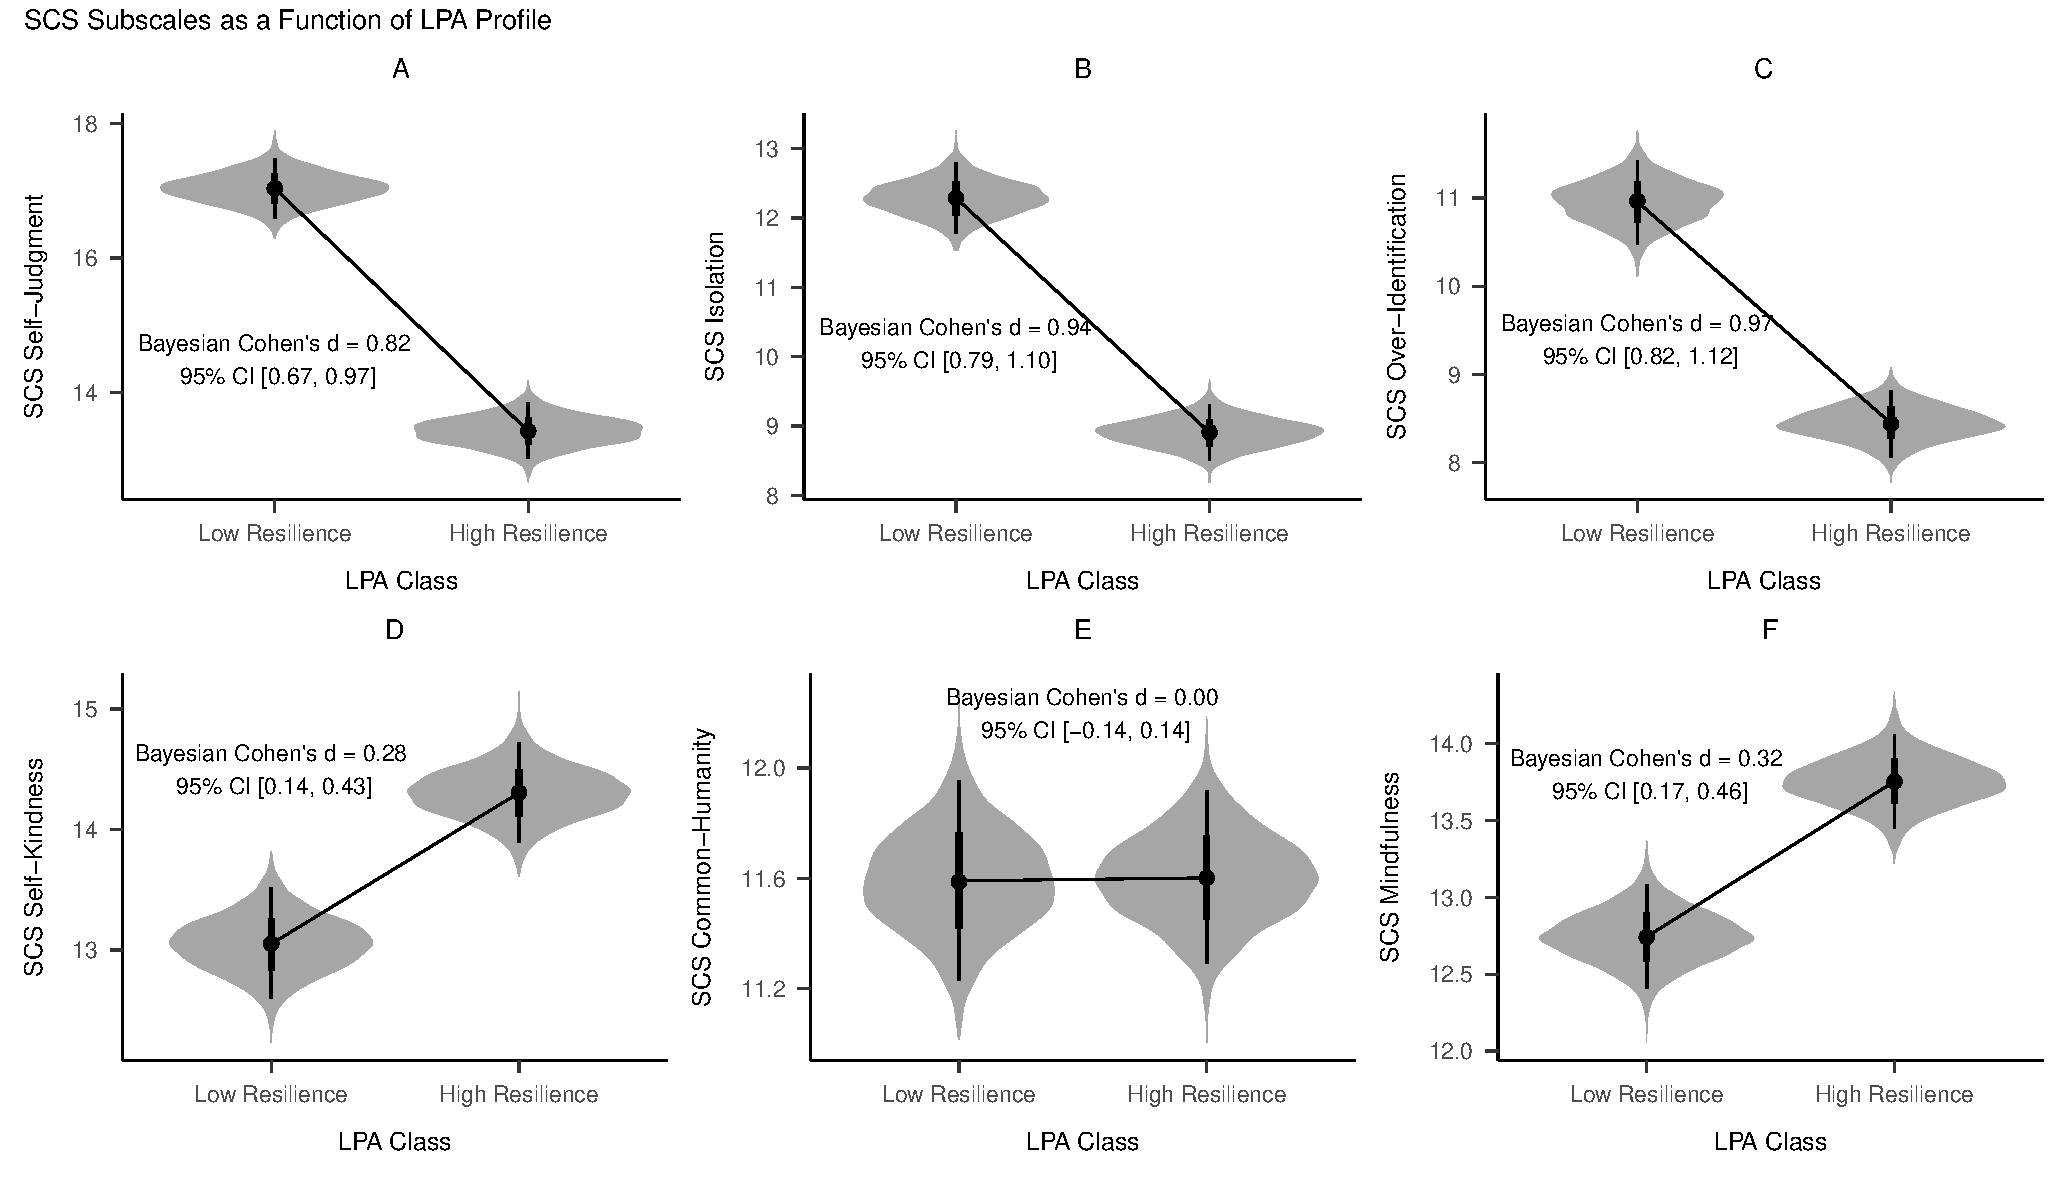
\includegraphics{figures/scs_subscales_lpa.pdf}
\caption{\label{fig:unnamed-chunk-1}My caption.}
\end{figure}

\hypertarget{discussion}{%
\section{Discussion}\label{discussion}}

The construct of self-compassion is commonly assessed using the Self-Compassion Scale (SCS) self-report questionnaire. The SCS measures six dimensions of self-compassion, three of which evaluate the active components of self-compassion. These dimensions include Self-kindness (SK), Common humanity (CH), and Mindfulness (MI), which involve being kind and understanding towards oneself, recognizing that personal failures and pain are common experiences, and maintaining awareness of one's painful thoughts and feelings. The remaining three dimensions evaluate the ``hindrances'' to self-compassion, including Self-judgment (SJ), Isolation (IS), and Overidentification (OI). These dimensions assess factors that hinder self-compassion, such as being self-critical and unsympathetic towards one's shortcomings, isolating oneself from others, and over-identifying with one's painful thoughts and emotions (Neff, 2022).

Compassion fatigue often leads to a sense of helplessness and a feeling of being unable to do more to help others (Boyle, 2015). This ``learned helplessness'' may lead individuals who experience compassion fatigue to rely more on non-self-compassionate coping strategies compared to those who are less affected by compassion fatigue (Gonzalez-Mendez \& Díaz, 2021).

decrease the use of self-compassionate responding (i.e., self-kindness, common humanity, mindfulness) and increase uncompassionate responding (i.e., self-judgment, isolation, overidentification) -- see also Gonzalez-Mendez and Díaz (2021).

We propose that individuals who experience compassion fatigue may not experience changes in compassionate responding, as their motivation to help others remains intact. However, they may experience a strong increase in uncompassionate responding (e.g., self-blaming), especially in those who are less directly involved in alleviating the suffering of others.

enabling an individual to mobilise internal resources and build up resistance against stressors

individuals with a strong SOC might experience reduced job stress.

\begin{center}\rule{0.5\linewidth}{0.5pt}\end{center}

Sense of coherence (SOC) originates from Antonovsky's (1979,
1987, 1991, 1993) theory of salutogenesis, a paradigm that focuses
on factors that promote health and well-being and considers the
salutary potential of stressors. SOC is a dispositional orientation that
reflects an individual's capacity to cope with life stressors and
comprises three components: Comprehensibility, the sense that
19
stimuli are predictable and structured (cognitive component);
Manageability, the sense that available resources (both internal and
external) are sufficient to cope with demands from the stimuli
(instrumental/behavioural component); and Meaningfulness, the
sense that the demands have significance and are worthy of
investment in terms of personal ideals and standards (motivational
component). An individual's SOC is reinforced by their ``general
resistance resources'' (e.g., intelligence, social support, coping
strategies, and preventative health orientation), which are shaped by
life experiences.

These results indicate the need for improving pre-employment strategies to select the most resilient individuals for rescue work, to implement continuous preventive measures for personnel.

\newpage

\hypertarget{references}{%
\section{References}\label{references}}

\hypertarget{refs}{}
\begin{CSLReferences}{1}{0}
\leavevmode\vadjust pre{\hypertarget{ref-afshar2015diagnostic}{}}%
Afshar-Oromieh, A., Avtzi, E., Giesel, F. L., Holland-Letz, T., Linhart, H. G., Eder, M., Eisenhut, M., Boxler, S., Hadaschik, B. A., Kratochwil, C., et al. (2015). The diagnostic value of PET/CT imaging with the 68 ga-labelled PSMA ligand HBED-CC in the diagnosis of recurrent prostate cancer. \emph{European Journal of Nuclear Medicine and Molecular Imaging}, \emph{42}, 197--209.

\leavevmode\vadjust pre{\hypertarget{ref-aldao2012adaptive}{}}%
Aldao, A., \& Nolen-Hoeksema, S. (2012). When are adaptive strategies most predictive of psychopathology? \emph{Journal of Abnormal Psychology}, \emph{121}(1), 276--281.

\leavevmode\vadjust pre{\hypertarget{ref-alexander2009first}{}}%
Alexander, D. A., \& Klein, S. (2009). First responders after disasters: A review of stress reactions, at-risk, vulnerability, and resilience factors. \emph{Prehospital and Disaster Medicine}, \emph{24}(2), 87--94.

\leavevmode\vadjust pre{\hypertarget{ref-angelini2023big}{}}%
Angelini, G. (2023). Big five model personality traits and job burnout: A systematic literature review. \emph{BMC Psychology}, \emph{11}(1), 1--35.

\leavevmode\vadjust pre{\hypertarget{ref-armstrong2004influence}{}}%
Armstrong-Stassen, M. (2004). The influence of prior commitment on the reactions of layoff survivors to organizational downsizing. \emph{Journal of Occupational Health Psychology}, \emph{9}(1), 46--60.

\leavevmode\vadjust pre{\hypertarget{ref-beck2016self}{}}%
Beck, A. T. (2016). \emph{The self in understanding and treating psychological disorders}. Cambridge University Press.

\leavevmode\vadjust pre{\hypertarget{ref-berger2012rescuers}{}}%
Berger, W., Coutinho, E. S. F., Figueira, I., Marques-Portella, C., Luz, M. P., Neylan, T. C., Marmar, C. R., \& Mendlowicz, M. V. (2012). Rescuers at risk: A systematic review and meta-regression analysis of the worldwide current prevalence and correlates of PTSD in rescue workers. \emph{Social Psychiatry and Psychiatric Epidemiology}, \emph{47}(6), 1001--1011.

\leavevmode\vadjust pre{\hypertarget{ref-bianchi2018burnout}{}}%
Bianchi, R. (2018). Burnout is more strongly linked to neuroticism than to work-contextualized factors. \emph{Psychiatry Research}, \emph{270}, 901--905.

\leavevmode\vadjust pre{\hypertarget{ref-boyle2015compassion}{}}%
Boyle, D. A. (2015). Compassion fatigue: The cost of caring. \emph{Nursing2022}, \emph{45}(7), 48--51.

\leavevmode\vadjust pre{\hypertarget{ref-burton2021individualism}{}}%
Burton, L., Delvecchio, E., Germani, A., \& Mazzeschi, C. (2021). Individualism/collectivism and personality in italian and american groups. \emph{Current Psychology}, \emph{40}, 29--34.

\leavevmode\vadjust pre{\hypertarget{ref-caprara2001brand}{}}%
Caprara, G. V., Barbaranelli, C., \& Guido, G. (2001). Brand personality: How to make the metaphor fit? \emph{Journal of Economic Psychology}, \emph{22}(3), 377--395.

\leavevmode\vadjust pre{\hypertarget{ref-carver1989assessing}{}}%
Carver, C. S., Scheier, M. F., \& Weintraub, J. K. (1989). Assessing coping strategies: A theoretically based approach. \emph{Journal of Personality and Social Psychology}, \emph{56}(2), 267--283.

\leavevmode\vadjust pre{\hypertarget{ref-chatzea2018ptsd}{}}%
Chatzea, V.-E., Sifaki-Pistolla, D., Vlachaki, S.-A., Melidoniotis, E., \& Pistolla, G. (2018). PTSD, burnout and well-being among rescue workers: Seeking to understand the impact of the european refugee crisis on rescuers. \emph{Psychiatry Research}, \emph{262}, 446--451.

\leavevmode\vadjust pre{\hypertarget{ref-cohen1985stress}{}}%
Cohen, S., \& Wills, T. A. (1985). Stress, social support, and the buffering hypothesis. \emph{Psychological Bulletin}, \emph{98}(2), 310--357.

\leavevmode\vadjust pre{\hypertarget{ref-connor2007relations}{}}%
Connor-Smith, J. K., \& Flachsbart, C. (2007). Relations between personality and coping: A meta-analysis. \emph{Journal of Personality and Social Psychology}, \emph{93}(6), 1080--1107.

\leavevmode\vadjust pre{\hypertarget{ref-costa1992normal}{}}%
Costa, P. T., \& McCrae, R. R. (1992). Normal personality assessment in clinical practice: The NEO personality inventory. \emph{Psychological Assessment}, \emph{4}(1), 5--13.

\leavevmode\vadjust pre{\hypertarget{ref-craparo2013impact}{}}%
Craparo, G., Faraci, P., Rotondo, G., \& Gori, A. (2013). The impact of event scale--revised: Psychometric properties of the italian version in a sample of flood victims. \emph{Neuropsychiatric Disease and Treatment}, \emph{9}, 1427--1432.

\leavevmode\vadjust pre{\hypertarget{ref-eriksson2013predeployment}{}}%
Eriksson, C. B., Lopes Cardozo, B., Foy, D. W., Sabin, M., Ager, A., Snider, L., Scholte, W. F., Kaiser, R., Olff, M., Rijnen, B., et al. (2013). Predeployment mental health and trauma exposure of expatriate humanitarian aid workers: Risk and resilience factors. \emph{Traumatology}, \emph{19}(1), 41--48.

\leavevmode\vadjust pre{\hypertarget{ref-gonzalez2021volunteers}{}}%
Gonzalez-Mendez, R., \& Díaz, M. (2021). Volunteers' compassion fatigue, compassion satisfaction, and post-traumatic growth during the SARS-CoV-2 lockdown in spain: Self-compassion and self-determination as predictors. \emph{Plos One}, \emph{16}(9), e0256854.

\leavevmode\vadjust pre{\hypertarget{ref-hobfoll1989conservation}{}}%
Hobfoll, S. E. (1989). Conservation of resources: A new attempt at conceptualizing stress. \emph{American Psychologist}, \emph{44}(3), 513--524.

\leavevmode\vadjust pre{\hypertarget{ref-joinson1992coping}{}}%
Joinson, C. (1992). Coping with compassion fatigue. \emph{Nursing}, \emph{22}(4), 116--118.

\leavevmode\vadjust pre{\hypertarget{ref-joormann2016examining}{}}%
Joormann, J., \& Stanton, C. H. (2016). Examining emotion regulation in depression: A review and future directions. \emph{Behaviour Research and Therapy}, \emph{86}, 35--49.

\leavevmode\vadjust pre{\hypertarget{ref-jung2022anxiety}{}}%
Jung, S., Sindermann, C., Yang, H., Elhai, J. D., \& Montag, C. (2022). Anxiety-related coping styles and individual differences in primary emotional systems against the background of affective neuroscience theory: A study using samples from germany and china. \emph{Trends in Psychology}, 1--17.

\leavevmode\vadjust pre{\hypertarget{ref-kokkinos2007job}{}}%
Kokkinos, C. M. (2007). Job stressors, personality and burnout in primary school teachers. \emph{British Journal of Educational Psychology}, \emph{77}(1), 229--243.

\leavevmode\vadjust pre{\hypertarget{ref-lanza2013latent}{}}%
Lanza, S. T., \& Rhoades, B. L. (2013). Latent class analysis: An alternative perspective on subgroup analysis in prevention and treatment. \emph{Prevention Science}, \emph{14}(2), 157--168.

\leavevmode\vadjust pre{\hypertarget{ref-lazarus1984stress}{}}%
Lazarus, R. S., \& Folkman, S. (1984). \emph{Stress, appraisal, and coping}. Springer publishing company.

\leavevmode\vadjust pre{\hypertarget{ref-liao2002association}{}}%
Liao, S.-C., Lee, M.-B., Lee, Y.-J., Weng, T., Shih, F.-Y., \& Ma, M. H. (2002). Association of psychological distress with psychological factors in rescue workers within two months after a major earthquake. \emph{Journal of the Formosan Medical Association}, \emph{101}(3), 169--176.

\leavevmode\vadjust pre{\hypertarget{ref-liu2017selection}{}}%
Liu, D. Y., \& Thompson, R. J. (2017). Selection and implementation of emotion regulation strategies in major depressive disorder: An integrative review. \emph{Clinical Psychology Review}, \emph{57}, 183--194.

\leavevmode\vadjust pre{\hypertarget{ref-lowery2022health}{}}%
Lowery, A., \& Cassidy, T. (2022). Health and well-being of first responders: The role of psychological capital, self-compassion, social support, relationship satisfaction, and physical activity. \emph{Journal of Workplace Behavioral Health}, \emph{37}(2), 87--105.

\leavevmode\vadjust pre{\hypertarget{ref-ludick2017toward}{}}%
Ludick, M., \& Figley, C. R. (2017). Toward a mechanism for secondary trauma induction and reduction: Reimagining a theory of secondary traumatic stress. \emph{Traumatology}, \emph{23}(1), 112--123.

\leavevmode\vadjust pre{\hypertarget{ref-lv2023influence}{}}%
Lv, G., Li, J., Xu, Q., Zhang, H., Wu, W., Fan, X., Wang, Z., \& Liu, H. (2023). The influence of firefighters' perceived stress on job burnout: A moderated mediation model. \emph{Current Psychology}, 1--11.

\leavevmode\vadjust pre{\hypertarget{ref-lyne2000psychometric}{}}%
Lyne, K., \& Roger, D. (2000). A psychometric re-assessment of the COPE questionnaire. \emph{Personality and Individual Differences}, \emph{29}(2), 321--335.

\leavevmode\vadjust pre{\hypertarget{ref-macbeth2012exploring}{}}%
MacBeth, A., \& Gumley, A. (2012). Exploring compassion: A meta-analysis of the association between self-compassion and psychopathology. \emph{Clinical Psychology Review}, \emph{32}(6), 545--552.

\leavevmode\vadjust pre{\hypertarget{ref-mao2022characteristics}{}}%
Mao, X., Fung, O. W., Hu, X., \& Loke, A. Y. (2022). Characteristics of resilience among disaster rescue workers: A systematic review. \emph{Disaster Medicine and Public Health Preparedness}, \emph{16}(1), 380--389.

\leavevmode\vadjust pre{\hypertarget{ref-mao2022concept}{}}%
Mao, X., Hu, X., \& Loke, A. Y. (2022). A concept analysis on disaster resilience in rescue workers: The psychological perspective. \emph{Disaster Medicine and Public Health Preparedness}, \emph{16}(4), 1682--1691.

\leavevmode\vadjust pre{\hypertarget{ref-marmar2006predictors}{}}%
Marmar, C. R., McCaslin, S. E., Metzler, T. J., Best, S., Weiss, D. S., Fagan, J., Liberman, A., Pole, N., Otte, C., Yehuda, R., et al. (2006). Predictors of posttraumatic stress in police and other first responders. \emph{Annals of the New York Academy of Sciences}, \emph{1071}(1), 1--18.

\leavevmode\vadjust pre{\hypertarget{ref-mirhaghi2016systematic}{}}%
Mirhaghi, A., Mirhaghi, M., Oshio, A., \& Sarabian, S. (2016). Systematic review of the personality profile of paramedics: Bringing evidence into emergency medical personnel recruitment policy. \emph{Eurasian Journal of Emergency Medicine}, \emph{15}(3), 144--149.

\leavevmode\vadjust pre{\hypertarget{ref-moritz2016more}{}}%
Moritz, S., Jahns, A. K., Schröder, J., Berger, T., Lincoln, T. M., Klein, J. P., \& Göritz, A. S. (2016). More adaptive versus less maladaptive coping: What is more predictive of symptom severity? Development of a new scale to investigate coping profiles across different psychopathological syndromes. \emph{Journal of Affective Disorders}, \emph{191}, 300--307.

\leavevmode\vadjust pre{\hypertarget{ref-murray2003neo}{}}%
Murray, G., Rawlings, D., Allen, N. B., \& Trinder, J. (2003). NEO five-factor inventory scores: Psychometric properties in a community sample. \emph{Measurement and Evaluation in Counseling and Development}, \emph{36}(3), 140--149.

\leavevmode\vadjust pre{\hypertarget{ref-naz2010development}{}}%
Naz, M., Saleem, S., \& Mahmood, Z. (2010). Development of indigenous resilience scale for rescue 1122 workers. \emph{Pakistan Journal of Psychological Research}, 149--163.

\leavevmode\vadjust pre{\hypertarget{ref-neff2003self}{}}%
Neff, K. D. (2003). Self-compassion: An alternative conceptualization of a healthy attitude toward oneself. \emph{Self and Identity}, \emph{2}(2), 85--101.

\leavevmode\vadjust pre{\hypertarget{ref-neff2022differential}{}}%
Neff, K. D. (2022). The differential effects fallacy in the study of self-compassion: Misunderstanding the nature of bipolar continuums. \emph{Mindfulness}, \emph{13}(3), 572--576.

\leavevmode\vadjust pre{\hypertarget{ref-neff2023self}{}}%
Neff, K. D. (2023). Self-compassion: Theory, method, research, and intervention. \emph{Annual Review of Psychology}, \emph{74}, 193--218.

\leavevmode\vadjust pre{\hypertarget{ref-norris1996received}{}}%
Norris, F. H., \& Kaniasty, K. (1996). Received and perceived social support in times of stress: A test of the social support deterioration deterrence model. \emph{Journal of Personality and Social Psychology}, \emph{71}(3), 498--511.

\leavevmode\vadjust pre{\hypertarget{ref-palm2004vicarious}{}}%
Palm, K. M., Polusny, M. A., \& Follette, V. M. (2004). Vicarious traumatization: Potential hazards and interventions for disaster and trauma workers. \emph{Prehospital and Disaster Medicine}, \emph{19}(1), 73--78.

\leavevmode\vadjust pre{\hypertarget{ref-paton2000disaster}{}}%
Paton, D., Smith, L., \& Violanti, J. (2000). Disaster response: Risk, vulnerability and resilience. \emph{Disaster Prevention and Management: An International Journal}, \emph{9}(3), 173--180.

\leavevmode\vadjust pre{\hypertarget{ref-pietrantoni2008resilience}{}}%
Pietrantoni, L., \& Prati, G. (2008). Resilience among first responders. \emph{African Health Sciences}, \emph{8}, 14--20.

\leavevmode\vadjust pre{\hypertarget{ref-pietrzak2014trajectories}{}}%
Pietrzak, R. H., Feder, A., Singh, R., Schechter, C. B., Bromet, E. J., Katz, C., Reissman, D., Ozbay, F., Sharma, V., Crane, M., et al. (2014). Trajectories of PTSD risk and resilience in world trade center responders: An 8-year prospective cohort study. \emph{Psychological Medicine}, \emph{44}(1), 205--219.

\leavevmode\vadjust pre{\hypertarget{ref-prati2014italian}{}}%
Prati, G., \& Pietrantoni, L. (2014). Italian adaptation and confirmatory factor analysis of the full and the short form of the posttraumatic growth inventory. \emph{Journal of Loss and Trauma}, \emph{19}(1), 12--22.

\leavevmode\vadjust pre{\hypertarget{ref-prezza2002rete}{}}%
Prezza, M., \& Principato, M. C. (2002). La rete sociale e il sostegno sociale. \emph{Conoscere La Comunit{à}}, 193--233.

\leavevmode\vadjust pre{\hypertarget{ref-ruaducu2022personality}{}}%
Răducu, C.-M., \& Stănculescu, E. (2022). Personality and socio-demographic variables in teacher burnout during the COVID-19 pandemic: A latent profile analysis. \emph{Scientific Reports}, \emph{12}(1), 14272.

\leavevmode\vadjust pre{\hypertarget{ref-scuri2019training}{}}%
Scuri, S., Petrelli, F., Nguyen, T., \& Grappasonni, I. (2019). Training to improve resilience and coping to monitor PTSD in rescue workers. \emph{Journal of Preventive Medicine and Hygiene}, \emph{60}(1), E58.

\leavevmode\vadjust pre{\hypertarget{ref-seery2011resilience}{}}%
Seery, M. D. (2011). Resilience: A silver lining to experiencing adverse life events? \emph{Current Directions in Psychological Science}, \emph{20}(6), 390--394.

\leavevmode\vadjust pre{\hypertarget{ref-setti2016role}{}}%
Setti, I., Lourel, M., \& Argentero, P. (2016). The role of affective commitment and perceived social support in protecting emergency workers against burnout and vicarious traumatization. \emph{Traumatology}, \emph{22}(4), 261--270.

\leavevmode\vadjust pre{\hypertarget{ref-sica2021facing}{}}%
Sica, C., Latzman, R. D., Caudek, C., Cerea, S., Colpizzi, I., Caruso, M., Giulini, P., \& Bottesi, G. (2021). Facing distress in coronavirus era: The role of maladaptive personality traits and coping strategies. \emph{Personality and Individual Differences}, \emph{177}, 110833.

\leavevmode\vadjust pre{\hypertarget{ref-sica2008coping}{}}%
Sica, C., Magni, C., Ghisi, M., Altoè, G., Sighinolfi, C., Chiri, L. R., \& Franceschini, S. (2008). Coping orientation to problems experienced-nuova versione italiana (COPE-NVI): Uno strumento per la misura degli stili di coping. \emph{Psicoterapia Cognitiva e Comportamentale}, \emph{14}(1), 27.

\leavevmode\vadjust pre{\hypertarget{ref-sica1997coping}{}}%
Sica, C., Novara, C., Dorz, S., \& Sanavio, E. (1997). Coping strategies: Evidence for cross-cultural differences? A preliminary study with the italian version of coping orientations to problems experienced (COPE). \emph{Personality and Individual Differences}, \emph{23}(6), 1025--1029.

\leavevmode\vadjust pre{\hypertarget{ref-swider2010born}{}}%
Swider, B. W., \& Zimmerman, R. D. (2010). Born to burnout: A meta-analytic path model of personality, job burnout, and work outcomes. \emph{Journal of Vocational Behavior}, \emph{76}(3), 487--506.

\leavevmode\vadjust pre{\hypertarget{ref-tahernejad2023post}{}}%
Tahernejad, S., Ghaffari, S., Ariza-Montes, A., Wesemann, U., Farahmandnia, H., \& Sahebi, A. (2023). Post-traumatic stress disorder in medical workers involved in earthquake response: A systematic review and meta-analysis. \emph{Heliyon}, e12794.

\leavevmode\vadjust pre{\hypertarget{ref-tedeschi1996posttraumatic}{}}%
Tedeschi, R. G., \& Calhoun, L. G. (1996). The posttraumatic growth inventory: Measuring the positive legacy of trauma. \emph{Journal of Traumatic Stress}, \emph{9}(3), 455--471.

\leavevmode\vadjust pre{\hypertarget{ref-thormar2016ptsd}{}}%
Thormar, S. B., Sijbrandij, M., Gersons, B. P., Van de Schoot, R., Juen, B., Karlsson, T., \& Olff, M. (2016). PTSD symptom trajectories in disaster volunteers: The role of self-efficacy, social acknowledgement, and tasks carried out. \emph{Journal of Traumatic Stress}, \emph{29}(1), 17--25.

\leavevmode\vadjust pre{\hypertarget{ref-veneziani2017self}{}}%
Veneziani, C. A., Fuochi, G., \& Voci, A. (2017). Self-compassion as a healthy attitude toward the self: Factorial and construct validity in an italian sample. \emph{Personality and Individual Differences}, \emph{119}, 60--68.

\leavevmode\vadjust pre{\hypertarget{ref-weiss2007impact}{}}%
Weiss, D. S. (2007). The impact of event scale: revised. In \emph{Cross-cultural assessment of psychological trauma and PTSD} (pp. 219--238). Springer.

\leavevmode\vadjust pre{\hypertarget{ref-wilson2019effectiveness}{}}%
Wilson, A. C., Mackintosh, K., Power, K., \& Chan, S. W. (2019). Effectiveness of self-compassion related therapies: A systematic review and meta-analysis. \emph{Mindfulness}, \emph{10}(6), 979--995.

\leavevmode\vadjust pre{\hypertarget{ref-wong2017self}{}}%
Wong, C. C. Y., \& Yeung, N. C. (2017). Self-compassion and posttraumatic growth: Cognitive processes as mediators. \emph{Mindfulness}, \emph{8}(4), 1078--1087.

\leavevmode\vadjust pre{\hypertarget{ref-zimet1988multidimensional}{}}%
Zimet, G. D., Dahlem, N. W., Zimet, S. G., \& Farley, G. K. (1988). The multidimensional scale of perceived social support. \emph{Journal of Personality Assessment}, \emph{52}(1), 30--41.

\end{CSLReferences}


\end{document}
